\chapter{进程}

    \emph{进程是任何躲到程序涉及的操作系统中的基本概念}

\section{进程、轻量级进程和线程}

    OS教科书的常规定义:\emph{进程是程序执行时的一个实例。}每一个进程都只有一个父亲。

    从内核的观点来看:\emph{进程的目的就是担当分配系统资源(CPU time、memory)的实体。}

    对于一个进程的创建,其原理是接受父进程地址空间的一个(逻辑)拷贝。\emph{尽管父子进程可以共享含有程序代码(正文)的页,但是拥有各自独立的数据拷贝,因此子进程对内存单元的修改对父进程是不可见的(反之亦然)}

    对于现代Unix系统来说,需要支持多线程应用————\emph{拥有很多相对独立执行流的用户程序共享应用的大部分数据结构。}这样的系统中,进程由多个线程组成,每个线程都代表进程的一个执行流。

    目前而言,大多数多线程应用都是基于pthread(POSIX thread)库的标准库函数集编写的

    Linux使用轻量级进程(lightweight process)对多线程进行更好的支持。\emph{对于轻量级进程而言,可以共享资源,只要其中一个修改共享资源,另一个就会立即查看并同步。}

\subsection{进程描述符}

    进程描述符(process descriptor,由task\_struct类修饰),其字段包含了与进程相关的所有信息。

\begin{figure}[!htbp]
    \centering
    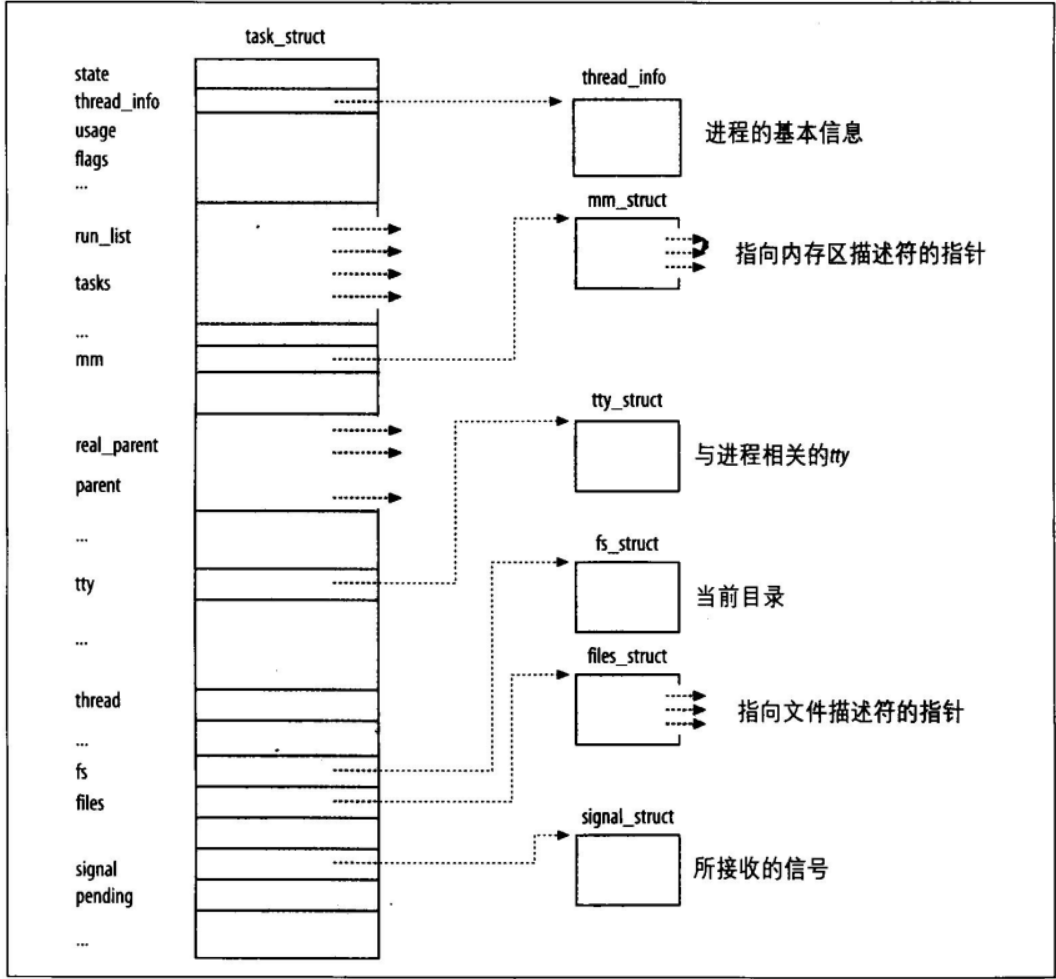
\includegraphics[width=0.8\textwidth]{image/chapter03/Linux进程描述符.png}
    \caption{Linux进程描述符}
\end{figure}

    图3-1右边的六个数据结构涉及进程拥有的所有特殊资源,目前我们只讨论两种:进程的状态以及进程的父子关系

\subsection{进程状态}

    进程描述符中的state字段描述了当前进程所处的状态。其由一组标志组成,其中每一个标志描述了一种可能的进程状态。

    值得注意的是:\emph{状态之间是互斥的,严格意义上只允许存在一种状态。}

\begin{lstlisting}[language=C++, caption={进程状态一览}]
#define TASK_RUNNING		    0
#define TASK_INTERRUPTIBLE	    1
#define TASK_UNINTERRUPTIBLE	2
#define TASK_STOPPED		    4
#define TASK_TRACED		        8
#define EXIT_ZOMBIE		        16
#define EXIT_DEAD		        32
\end{lstlisting}

\begin{itemize}
    \item TASK\_RUNNING
    \subitem 进程要么已经执行,要么准备执行
    \item TASK\_INTERRUPTIBLE
    \subitem 进程被挂起,知道某个条件为真。产生硬件中断,释放进程正在等待的系统资源或传递一个信号都是可以唤醒进程的条件(也就是恢复到TASK\_RUNNING)
    \item TASK\_UNINTERRUPTIBLE
    \subitem 与上一个状态类似,但传递信号无法唤醒。\emph{一般用于特殊情况下,进程必须等待,直到一个不能被中断的实践发生}
    \item TASK\_STOPPED
    \subitem 进程的执行被暂停,当接收到SIGSTOP、SIGTSTP、SIGTTIN和SIGTTOU信号后,进入暂停
    \item TASK\_TRACED
    \subitem 进程的执行由debugger程序暂停。当一个进程被另一个进程监控时,任何信号都可以把这个进程置于TASK\_TRACED状态
    \item EXIT\_ZOMBIE
    \subitem 进程的执行被终止,但是父进程未发布wait()类系统调用来返回有关死亡进程的信息
    \item EXIT\_DEAD
    \subitem 最终状态,由于父进程刚发布wait()类系统调用,因而进程被系统删除,但防止其他线程也执行wait()类系统调用,为了防止冲突,因而将僵死状态设置为僵死撤销(将亡)状态
\end{itemize}

    一般的,进程状态可以由以下简单的赋值语句设置,也可以由宏设置:

\begin{lstlisting}[language=C++]
p->state = TASK_RUNNING;

#define __set_task_state(tsk, state_value)		\
	do { (tsk)->state = (state_value); } while (0)
#define set_task_state(tsk, state_value)		\
	set_mb((tsk)->state, (state_value))

#define __set_current_state(state_value)			\
	do { current->state = (state_value); } while (0)
#define set_current_state(state_value)		\
	set_mb(current->state, (state_value))
\end{lstlisting}

\subsection{标识一个进程}

    进程和进程描述符之间有非常严格的一一对应关系,这使得进程描述符标识进程称为一种方便的方式。

    另一方面,类Unix操作系统允许用户使用进程标识符process ID(PID)来标识进程,PID存放在进程描述符的pid字段中。

    PID被顺序编号,新创建的进程通常是前一个PID加1。PID的值通常有一个上线,缺省情况下,最大PID号是32767(PID\_MAX\_DEFAULT - 1)

    由于循环使用PID,因此需要通过与个pidmap\_array位图来标识当前已分配的PID和闲置的PID。

    Linux希望同一个线程组内有同一个PID,因此,\emph{一个线程组中的所有线程使用和该线程组的领头线程的PID,被存放在进程描述符中的tgid字段。}系统调用getpid()实际上是返回的tgid的值,而非PID。

\subsection{进程描述符处理}

    进程是动态实体,因此内核必须能够同时处理多进程,并把进程描述符存放在动态内存中,而非在永久分配给内核的内存区。

    对于每个进程来说,Linux把内核态的进程堆栈和进程描述符中的thread\_info(线程描述符)紧凑的存放在一个单独的存储区域内。

\begin{figure}[!htbp]
    \centering
    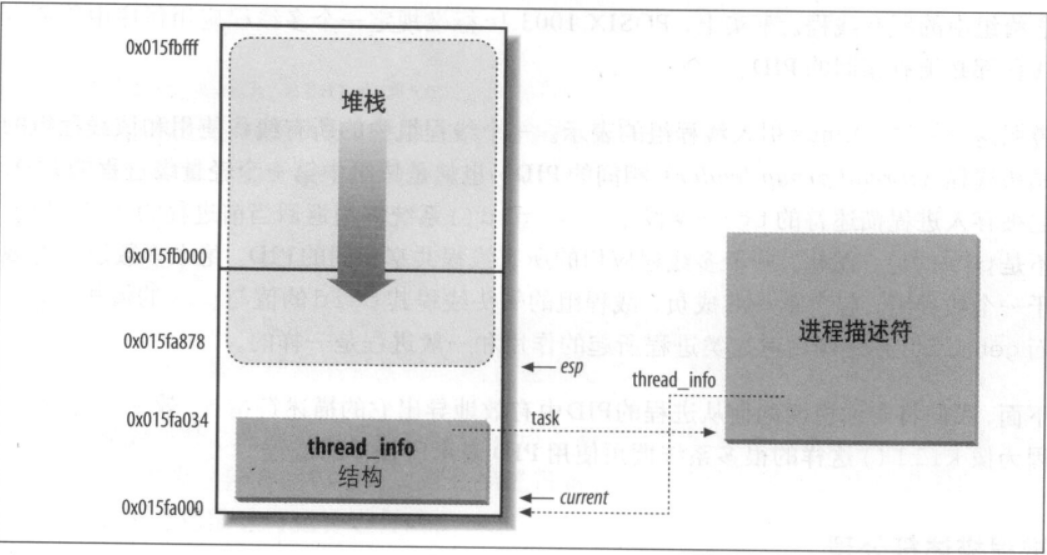
\includegraphics[width=0.8\textwidth]{image/chapter03/thread_info与进程内核栈.png}
    \caption{thread\_info结构和进程内核栈存放在两个连续的页框中}
\end{figure}

    线程描述符驻留于该内存区的开始,栈从末端向下开始增长。

    esp寄存器是CPU的栈指针(x86架构),用来存放栈顶单元的地址。栈起始于末端,并朝该内存区开始的地方开始增长。\emph{从用户态切换到内核态后,进程的内核总是空的}

    在内核中,使用union对该结构进行描述:

\begin{lstlisting}[language=C++]
#define THREAD_SIZE     (4096)
#else
#define THREAD_SIZE		(8192)
#endif

union thread_union {
    struct thread_info thread_info;
    unsigned long stack[THREAD_SIZE/sizeof(long)];
};
\end{lstlisting}

\subsection{标识当前进程}

    从效率上看:\emph{thread\_info结构体与内核态堆栈之间的紧密结合提供的主要好处为:内核可以轻易从esp的值获取CPU正在运行进程的thread\_info的地址}

    事实上,如果thread\_union结构长度是8K($2^{13}$),则内核屏蔽掉esp的低13位有效位就能够获取thread\_info的基地址。这项工作由以下函数实现:

\begin{lstlisting}[language=C++]
/* how to get the thread information struct from C */
static inline struct thread_info *current_thread_info(void)
{
    struct thread_info *ti;
    __asm__("andl %%esp,%0; ":"=r" (ti) : "0" (~(THREAD_SIZE - 1)));
    return ti;
}
\end{lstlisting}

    也就是说,通过该函数内联汇编:

\begin{lstlisting}[language=C++]
movl $0xffffe000, %ecx
andl %esp, %ecx
movl %ecx, p
\end{lstlisting}

    这样执行后,p就包含了CPU当前运行进程的thread\_info结构的指针。

    但是,进程中最常用的是进程描述符的地址而非thread\_info的地址,因此,内核需要调用current宏,其等价于

\begin{lstlisting}[language=C++]
current_thread_info()->task;

movl $0xffffe000, %ecx
andl %esp, %ecx
movl (%ecx), p
\end{lstlisting}

    查看源码可以知道,task在thread\_info上的偏移量是0,因此上述三条指令就能够将进程描述符指针赋值到p上。

\subsection{双向链表}

    对于每一个链表,都需要实现一组原语操作:初始化,插入和删除,遍历等操作。Linux内核定义了list\_head数据结构,字段next和prev分别表示通用黄翔链表向前和向后的指针元素。

\begin{lstlisting}[language=C++]
struct list_head {
    struct list_head *next, *prev;
};
\end{lstlisting}

\begin{figure}[!htbp]
    \centering
    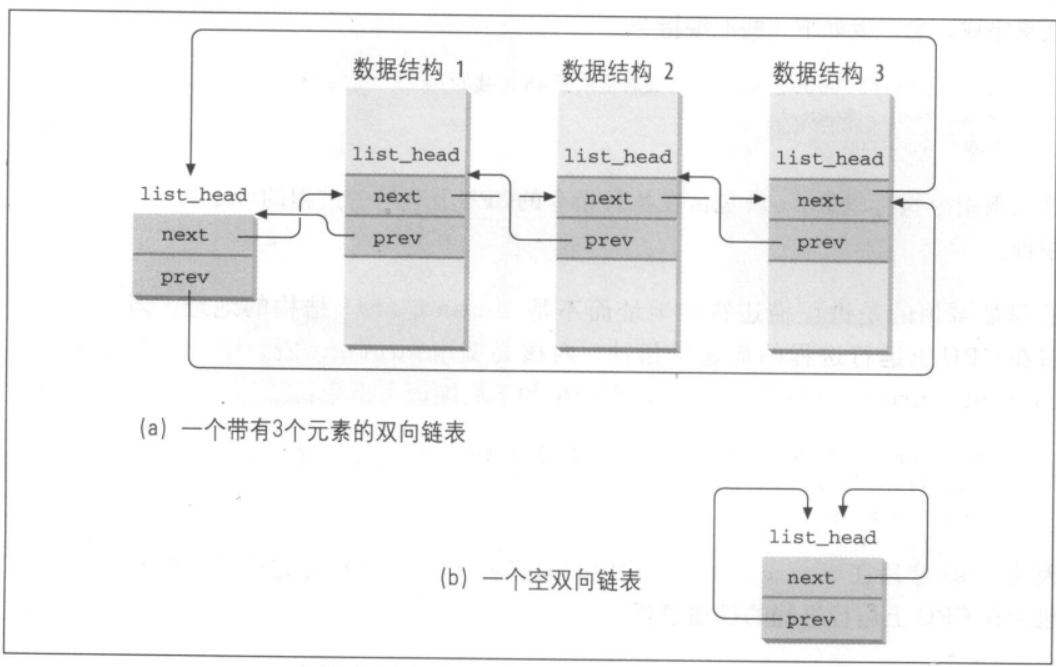
\includegraphics[width=0.6\textwidth]{image/chapter03/list_head构造双向链表.png}
    \caption{list\_head构造双向链表}
\end{figure}

    对于新链表而言,是用LIST\_HEAD(list\_name)宏创建的,其声明类型为list\_head的新变量list\_name。见上图中b图。Linux内核为链表提供了一些原语操作:

\begin{lstlisting}[language=C++]
// 初始化链表
#define LIST_HEAD_INIT(name) { &(name), &(name) }
#define LIST_HEAD(name) \
    struct list_head name = LIST_HEAD_INIT(name)
// 链表头插
static inline void list_add(
    struct list_head *new, struct list_head *head)
{
    __list_add(new, head, head->next);
}
// 链表尾插
static inline void list_add_tail(
    struct list_head *new, struct list_head *head)
{
	__list_add(new, head->prev, head);
}
// 链表删除
static inline void list_del(struct list_head *entry)
{
	__list_del(entry->prev, entry->next);
	entry->next = LIST_POISON1;
	entry->prev = LIST_POISON2;
}
// 链表判空
static inline int list_empty(const struct list_head *head)
{
	return head->next == head;
}
// 获取链表元素
#define list_entry(ptr, type, member) \
	container_of(ptr, type, member)
// 遍历链表
#define list_for_each(pos, head) \
for (pos = (head)->next; prefetch(pos->next), pos != (head); \
        pos = pos->next)

#define list_for_each_entry(pos, head, member)				\
for (pos = list_entry((head)->next, typeof(*pos), member);	\
        prefetch(pos->member.next), &pos->member != (head); 	\
        pos = list_entry(pos->member.next, typeof(*pos), member))
\end{lstlisting}

\subsubsection{进程链表}

    进程链表把所有的进程描述符链接起来。每一个task\_struct结构都包含一个list\_head类型的tasks字段,prev和next分贝指向前后的task\_struct元素。

    进程链表的头是init\_struct描述符,也就是0进程(process 0)或swapper进程的进程描述符。

    SET\_LINKS和REMOVE\_LINKS分别用于从进程链表中插入和删除一个进程描述符,且考虑了父子进程间关系。同时也有宏for\_each\_process,遍历整个进程链表。

\begin{lstlisting}[language=C++]
#define next_task(p)	\
    list_entry((p)->tasks.next, struct task_struct, tasks)
#define prev_task(p)	\
    list_entry((p)->tasks.prev, struct task_struct, tasks)
#define for_each_process(p) \
    for (p = &init_task ; (p = next_task(p)) != &init_task ; )
\end{lstlisting}

\subsubsection{TASK\_RUNNING状态的进程链表}

    当内核寻找新进程运行时,\emph{只需要考虑处于TASK\_RUNNING状态的进程}

    早先的Linux把可运行进程都放在运行队列(runqueue)的链表中,但是维持链表中进程优先级排序的开销过大,因此早期的调度程序不得不为选择最佳可运行程序而扫描整个进程。

    而2.6实现的运行队列,目的是为了\emph{让调度程序在固定时间内选出最佳可运行进程,与队列中可运行的进程数无关。}

    \emph{提高调度程序运行速度的诀窍是建立多个可运行进程链表,每种进程优先级对应一个不同的链表。}

    每个task\_struct描述符包含一个list\_head类型的字段run\_list,如果进程优先级等于k(取值为0~139),run\_list就把该进程链入优先级为k的可运行进程队列中。

    在内核中,运行队列的主要数据结构还是组成运行队列的进程描述符链表,所有这些链表都由一个单独prio\_array\_t数据结构来实现

\begin{lstlisting}[language=C++]
struct prio_array {
    // 链表中进程描述符的数量
    unsigned int nr_active;
    // 优先权位图,仅当某个优先权的进程链表不为空时设置
    unsigned long bitmap[BITMAP_SIZE];
    // 140个优先权队列的头节点
    struct list_head queue[MAX_PRIO];
};

typedef struct prio_array prio_array_t;

static void enqueue_task(struct task_struct *p, prio_array_t *array)
{
	sched_info_queued(p);
	list_add_tail(&p->run_list, array->queue + p->prio);
	__set_bit(p->prio, array->bitmap);
	array->nr_active++;
	p->array = array;
}
\end{lstlisting}

    enqueue\_task把进程描述符插入某个运行队列的链表,进程描述符的prio字段存放进程的动态优先权,array时一个指针,指向当前队列的prio\_array\_t数据结构。

\subsection{进程间的关系}

    程序创建的进程具有父/子关系,而一个进程创建多个子进程,子进程之间具有兄弟关系。

    因此,进程描述符中引入几个字段表示这些关系。\emph{进程0和进程1由内核创建}

\begin{lstlisting}[language=C++]
/* real parent process (when being debugged) */
struct task_struct *real_parent; 
struct task_struct *parent;	/* parent process */
/*
* children/sibling forms the list of my children plus the
* tasks I'm ptracing.
*/
/* list of my children */
struct list_head children;	
/* linkage in my parent's children list */
struct list_head sibling;	
\end{lstlisting}

    下图中演示了一组进程间的关系:

\begin{figure}[!htbp]
    \centering
    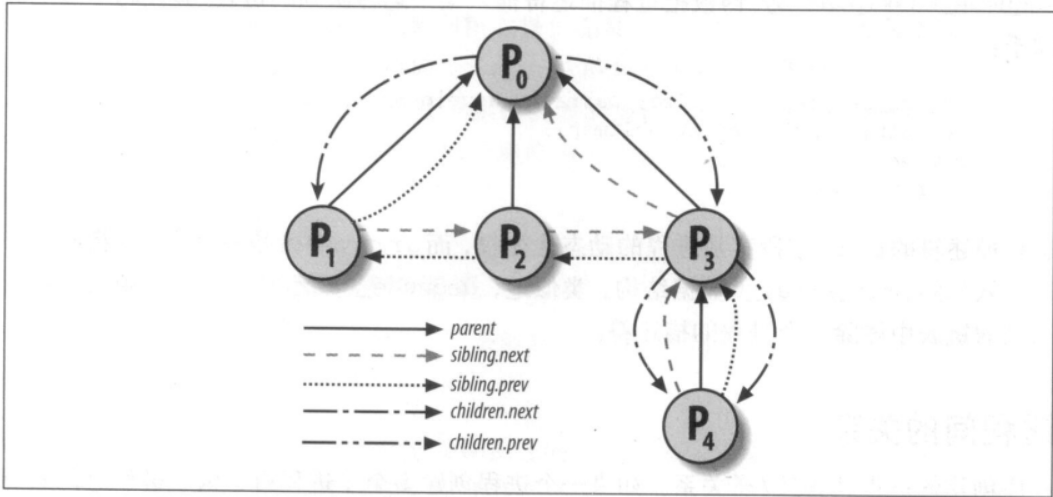
\includegraphics[width=0.8\textwidth]{image/chapter03/五个进程间的亲属关系.png}
    \caption{五个进程间的亲属关系}
\end{figure}

    值得注意的是,\emph{一个进程可能是一个进程组或登录会话的领头进程,也可能是线程组的临潼进程,还可能是跟踪其他进程执行}

\begin{lstlisting}[language=C++]
group_leader        // P所在进程组的领头进程描述符指针
signal->pgrp        // P所在进程组的领头进程PID
tgid                // P所在线程组的领头进程PID
signal->session     // P的登录会话领头进程PID
ptrace_children     // 链表头部,包含所有被debugger程序跟踪子线程
ptrace_list         // 跟踪进程父进程链表的前后元素
\end{lstlisting}

\subsubsection{pidhash表及链表}

    在一些情况下,内核必须从进程的PID导出对应的进程描述符指针:为kill()系统调用提供服务

    顺序扫描进程链表并检查进程描述符PID的做法可行,但是相当低效。为了快速查找,引入了4个散列表。引入4个散列表的原因是:进程描述符包含了表示不同类型的PID字段,每种PID都需要自己的散列表

\begin{table*}[!htbp]
    \begin{center}
        \caption{散列表和进程描述符中的相关字段}
        \begin{tabular}{c c c}
            \hline
            Hash表的类型 & 字段名 & 说明 \\
            PIDTYPE\_PID & pid & 进程的PID \\
            PIDTYPE\_TGID & tgid & 进程组领头进程的PID \\
            PIDTYPE\_PGID & pgrp & 线程组领头进程的PID \\
            PIDTYPE\_SID & session & 会话领头进程的PID \\
            \hline
        \end{tabular}
    \end{center}
\end{table*}

    \emph{内核初始化期间动态地为4个散列表分配空间,并把它们的地址存入pid\_hash数组}

    用pid\_hashfn宏把PID转化为表索引:

\begin{lstlisting}[language=C++]
#if BITS_PER_LONG == 32
/* 2^31 + 2^29 - 2^25 + 2^22 - 2^19 - 2^16 + 1 */
#define GOLDEN_RATIO_PRIME 0x9e370001UL
#elif BITS_PER_LONG == 64
/*  2^63 + 2^61 - 2^57 + 2^54 - 2^51 - 2^18 + 1 */
#define GOLDEN_RATIO_PRIME 0x9e37fffffffc0001UL
#else
#error Define GOLDEN_RATIO_PRIME for your wordsize.
#endif

#define pid_hashfn(nr) hash_long((unsigned long)nr, pidhash_shift)

static inline unsigned long hash_long(unsigned long val, unsigned int bits)
{
	unsigned long hash = val;

#if BITS_PER_LONG == 64
	/*  Sigh, gcc can't optimise this alone like it does for 32 bits. */
	unsigned long n = hash;
	n <<= 18; hash -= n;
	n <<= 33; hash -= n;
	n <<= 3; hash += n;
	n <<= 3; hash -= n;
	n <<= 4; hash += n;
	n <<= 2; hash += n;
#else
	/* On some cpus multiply is faster, on others gcc will do shifts */
	hash *= GOLDEN_RATIO_PRIME;
#endif

	/* High bits are more random, so use them. */
	return hash >> (BITS_PER_LONG - bits);
}
\end{lstlisting}

    但是,我们清楚:\emph{散列(hash)函数并不总能确保PID与表的索引一一对应,两个不同的PID散列到相同的表索引被称为冲突(colliding)}

    Linux利用链表来处理冲突的PID:\emph{每个表项是由冲突的进程描述符组成的双向链表}

\begin{figure}[!htbp]
    \centering
    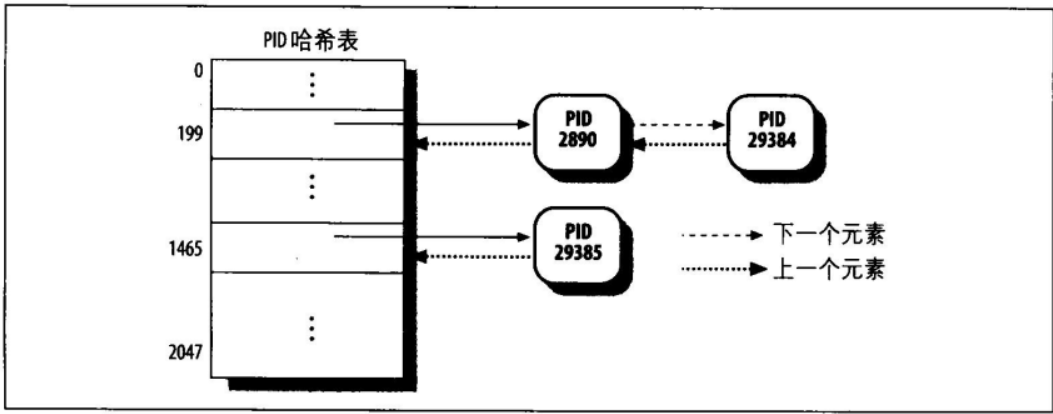
\includegraphics[width=0.8\textwidth]{image/chapter03/pidhash表及链表.png}
    \caption{pidhash表及链表}
\end{figure}

    可以看见,PID2890和PID29384被散列到第200的元素处,然后通过双向链表进行链接。

    \emph{具有链表的散列法比PID到表索引的线性转换更为优越,因为系统中的进程数总是远远小于32768。}

    PID散列表的数据结构解决了上述的难题,最主要的数据结构是四个PID结构的素组,其在进程描述符的PID字段中:

\begin{lstlisting}[language=C++]
enum pid_type
{
	PIDTYPE_PID,
	PIDTYPE_TGID,
	PIDTYPE_PGID,
	PIDTYPE_SID,
	PIDTYPE_MAX
};

struct pid
{
    // pid的数值
	int nr;
    // 链接散列表的前后元素
	struct hlist_node pid_chain;
	// 每一个pid的进程链表头
	struct list_head pid_list;
};
\end{lstlisting}

\begin{figure}[!htbp]
    \centering
    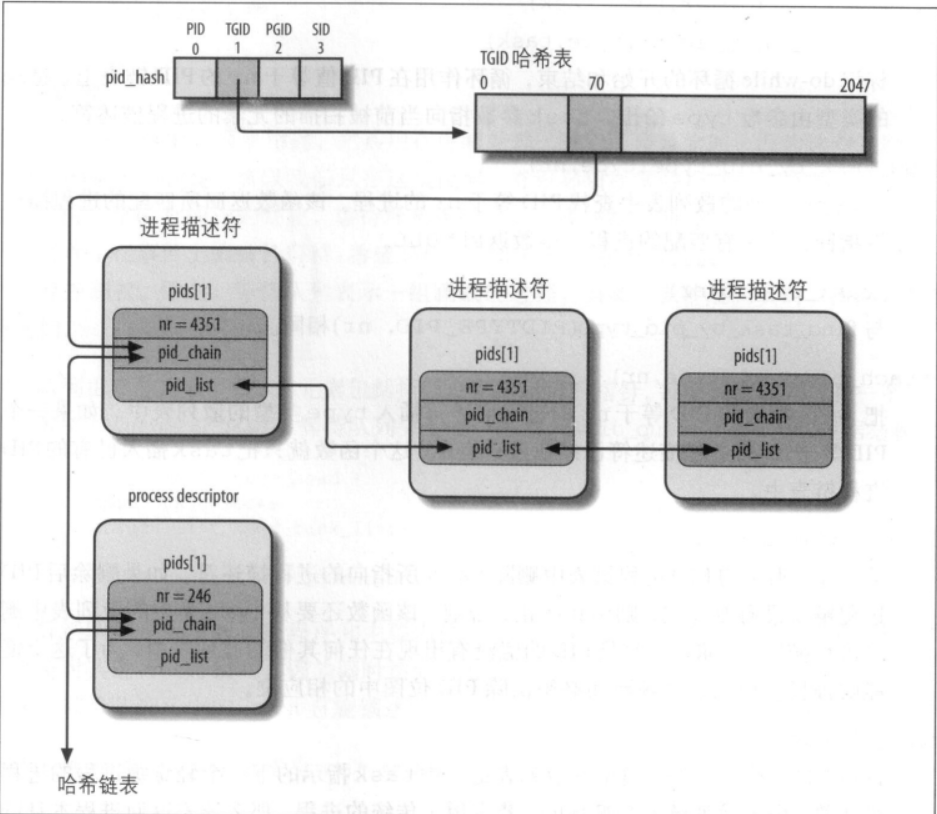
\includegraphics[width=0.8\textwidth]{image/chapter03/pid散列表.png}
    \caption{pid散列表}
\end{figure}

    下面是处理PID散列表的函数和宏:

\begin{itemize}
    \item do\_each\_task\_pid(who, type, task)
    \item while\_each\_task\_pid(who, type, task)
    \subitem 循环作用在PID值等于nr的PID链表上,类型由type给出,task参数指出当前被扫描的元素的进程描述符
    \item task\_t *find\_task\_by\_pid\_type(int type, int nr)
    \subitem 在type类型的散列表中查找pid等于nr的进程,返回所匹配的进程描述符指针
    \item find\_task\_by\_pid(nr)
    \item int fastcall attach\_pid(task\_t *task, enum pid\_type type, int nr)
    \subitem 把task指向的PID等于nr的进程描述符插入type类型的散列表中。如果已经存在,则只把task插入已有PID的进程链表
    \item void fastcall detach\_pid(task\_t *task, enum pid\_type type)
    \subitem 删除task所指向的进程描述符,若删除后链表未变空,则函数终止;否则还要从type类型的散列表中删除进程描述符,若该PID在任何散列表中不存在,则清除PID位图中的对应位
    \item task\_t fastcall *next\_thread(const task\_t *p)
    \subitem 返回TGID类型中的散列表链接中task知识的下一个轻量级进程的进程描述符
\end{itemize}

\subsection{如何组织进程}

    运行队列链表把处于TASK\_RUNNING状态的所有进程都组织再一起,但对于其他状态:

\begin{itemize}
    \item 没有为TASK\_STOPPED、EXIT\_ZOMBIE或EXIT\_DEAD状态的进程专门建立链表
\end{itemize}

\subsubsection{等待队列}    

    \emph{等待队列再中断处理、进程同步和定时方面尤为重要。}

    进程必须经常等待某些事件的发生,例如的带一个磁盘操作的弘治,的带释放系统资源,或等待时间经过固定的间隔。等待队列实现了在事件上的等待

    \emph{希望等待特定的事件的进程将自己放入合适的等待队列,并放弃控制权,一旦某条件为真,由内核唤醒。} 

    等待队列由双向列表实现,其元素包括指向进程描述符的指针

\begin{lstlisting}[language=C++]
struct __wait_queue_head {
    spinlock_t lock;
    struct list_head task_list;
};
typedef struct __wait_queue_head wait_queue_head_t;

struct __wait_queue {
	unsigned int flags;
#define WQ_FLAG_EXCLUSIVE	0x01
	struct task_struct * task;
	wait_queue_func_t func;
	struct list_head task_list;
};
typedef struct __wait_queue wait_queue_t;
\end{lstlisting}

    等待队列是由中断处理程序和主要内核函数修改而来,因此必须对该链表进程保护以免被同时访问,因此通过自旋锁来确保。

    等待队列链表中的每个元素代表一个睡眠进程,该进程等待某一事件的发生。然而要唤醒等待队列中的所有睡眠进程有时并不方便,因此有两种睡眠进程。

    互斥进程(等待队列元素的flags字段为1)由内核有选择地唤醒;而非互斥进程(flags值为0)总是由内核在事件发生时唤醒。

\subsubsection{等待队列的操作}

\begin{lstlisting}[language=C++]
#define __WAITQUEUE_INITIALIZER(name, tsk) {				\
.task		= tsk,						\
.func		= default_wake_function,			\
.task_list	= { NULL, NULL } }

#define DECLARE_WAITQUEUE(name, tsk)					\
	wait_queue_t name = __WAITQUEUE_INITIALIZER(name, tsk)
\end{lstlisting}

    可以用DECLEAR\_WAIT\_QUEUE\_HEAD宏定义一个新等待队列的头,其静态声明一个叫name的等待队列的头变量并对该变量的lock和task\_list字段进行初始化。

    函数init\_waitqueue\_head()可以用来初始化动态分配的等待队列的头变量

\begin{lstlisting}[language=C++]
static inline void init_waitqueue_head(wait_queue_head_t *q)
{
    q->lock = SPIN_LOCK_UNLOCKED;
    INIT_LIST_HEAD(&q->task_list);
}
\end{lstlisting}

    非互斥进程将由default\_wake\_function()唤醒。

    一旦定义了一个元素,必须将其插入等待队列,add\_wait\_queue()函数把一个非互斥进程插入等待队列链表的第一个位置。add\_wait\_queue\_exclusive()函数把一个互斥进程插入等待队列的最后一个位置。

\begin{lstlisting}[language=C++]
static inline void __add_wait_queue(
    wait_queue_head_t *head, wait_queue_t *new)

static inline void add_wait_queue_exclusive_locked(
    wait_queue_head_t *q, wait_queue_t *wait)
\end{lstlisting}

    要等待特定条件的进程可以调用如下中的任何一个函数:

\begin{itemize}
    \item void fastcall \_\_sched sleep\_on(wait\_queue\_head\_t *q)
    \subitem 该函数把当前进程状态设置为TASK\_UNINTERRUPTIBLE,并把其插入到特定的等待队列。然后调度程序重新开始另一个程序的执行
    \subitem 当睡眠进程被唤醒,则调度程序重新执行sleep\_on()函数,并把该进程从队列中删除
    \item \_\_sched interruptible\_sleep\_on\_timeout(wait\_queue\_head\_t *q, long timeout)
    \subitem 和上一个函数类似,但该函数将状态设置为TASK\_INTERRUPTIBLE,因此接受一个信号就可以唤醒当前进程
    \item long fastcall \_\_sched sleep\_on\_timeout(wait\_queue\_head\_t *q, long timeout)
    \subitem 和上一个函数类似,但其允许定义一个时间间隔,过了该间隔,由内核唤醒,因此调用schedule\_timeout()函数
    \item 在2.6kernel下引入了prepare\_to\_wait()、prepare\_to\_wait\_exclusive()和finish\_wait(),提供了另一种途径来使当前进程在一个等待队列中睡眠
\end{itemize}

\begin{lstlisting}[language=C++]
void fastcall prepare_to_wait(
    wait_queue_head_t *q, wait_queue_t *wait, int state)
void fastcall prepare_to_wait_exclusive(
    wait_queue_head_t *q, wait_queue_t *wait, int state)
void fastcall finish_wait(wait_queue_head_t *q, wait_queue_t *wait)

DEFINE_WAIT(wait);
prepare_to_wait_exclusive(&wq, &wait, TASK_INTERRUPTIBLE);
...
if (!condition)
    schedule();
finish_wait(&wq, &wait);
\end{lstlisting}

    prepare\_to\_wait()和prepare\_to\_wait\_exclusive()中的第三个参数设置进程的状态,然后把等待队列元素的互斥标志flag设置为0或1,最后把等待元素wait插入到wq为头的等待队列的链表中。

    wait\_event和wait\_event\_interruptible宏使它们的调用进程在等待队列上睡眠,一直到修改了给定条件为止

\begin{lstlisting}[language=C++]    
#define __wait_event(wq, condition) 					\
do {									\
	DEFINE_WAIT(__wait);						\
									\
	for (;;) {							\
		prepare_to_wait(&wq, &__wait, TASK_UNINTERRUPTIBLE);	\
		if (condition)						\
			break;						\
		schedule();						\
	}								\
	finish_wait(&wq, &__wait);					\
} while (0)

#define wait_event(wq, condition) 					\
do {									\
    if (condition)	 						\
        break;							\
    __wait_event(wq, condition);					\
} while (0)
\end{lstlisting}

    值得注意的使:\emph{sleep\_on()类函数在以下条件下不能使用,那就是必须测试条件且该条件还没有得到验证时,又让进程去睡眠,这样是竞争条件产生的根源。}

    内核可以通过下面任何一个宏唤醒等待队列中的进程并把其状态设置为RUNNING:wake\_up、wake\_up\_nr、wake\_up\_all、wake\_up\_interruptible、wake\_up\_interruptible\_nr、wake\_up\_interruptible\_all、wake\_up\_interruptible\_sync、wake\_up\_locked。

\begin{itemize}
    \item 所有宏都考虑到处于INTERRUPTIBLE状态的睡眠进程;若宏的名字中不含"interruptible",那么处于UNINTERRUPTIBLE的进程也会被考虑到
    \item 所有宏都具有唤醒请求状态的所有非互斥进程
    \item 名字中含有"nr"字符串的宏唤醒给定数具有请求状态的互斥进程;"all"唤醒所有具有请求状态的互斥进程,都不含的唤醒一个互斥进程
    \item 名字中不含"snyc"的宏检查被唤醒进程的优先级是否高于系统中正在运行的进程优先级,并在必要时调用schedule()
    \item wake\_up\_locked需要自旋锁被持有
\end{itemize}

\begin{lstlisting}[language=C++]
void fastcall __wake_up(wait_queue_head_t *q, unsigned int mode,
    int nr_exclusive, void *key)
{
    unsigned long flags;

    spin_lock_irqsave(&q->lock, flags);
    __wake_up_common(q, mode, nr_exclusive, 0, key);
    spin_unlock_irqrestore(&q->lock, flags);
} 
#define wake_up(x)			\
    __wake_up(              \
        x, TASK_UNINTERRUPTIBLE | TASK_INTERRUPTIBLE, 1, NULL)
\end{lstlisting}

\subsection{进程资源限制}

    \emph{每一个进程都有一组相关的资源限制(resource limit),限定了进程能使用的系统资源数论。}

\begin{lstlisting}[language=C++]
/* Allow arch to control resource order */
#ifndef __ARCH_RLIMIT_ORDER
#define RLIMIT_CPU		    0	/* CPU time in ms */
#define RLIMIT_FSIZE		1	/* Maximum filesize */
#define RLIMIT_DATA		    2	/* max data size */
#define RLIMIT_STACK		3	/* max stack size */
#define RLIMIT_CORE		    4	/* max core file size */
#define RLIMIT_RSS		    5	/* max resident set size */
#define RLIMIT_NPROC		6	/* max number of processes */
#define RLIMIT_NOFILE		7	/* max number of open files */
#define RLIMIT_MEMLOCK		8	/* max locked-in-memory address space */
#define RLIMIT_AS		    9	/* address space limit */
#define RLIMIT_LOCKS		10	/* maximum file locks held */
#define RLIMIT_SIGPENDING	11	/* max number of pending signals */
#define RLIMIT_MSGQUEUE		12	/* maximum bytes in POSIX mqueues */

#define RLIM_NLIMITS		13
#endif
\end{lstlisting}

    对当前进程的资源限制存放在current->signal->rlim字段中,即进程的信号描述符的一个字段,该字段是类型为rlimit结构的数组

\begin{lstlisting}[language=C++]
struct rlimit {
    unsigned long	rlim_cur;
    unsigned long	rlim_max;
};
\end{lstlisting}

    rlim\_cur是当前资源限制,rlim\_max是资源限制所允许的最大值。

    利用getrlimit()和setrlimit()系统调用,用户能够把一些资源的rlim\_cur限制增加。\emph{当然的,只有管理员权限才能使用。}

\section{进程切换}

    \emph{为了控制进程的执行,内核必须有能力挂起CPU上允许的进程,并恢复以前挂起某个进程的执行,这种行为被称为进程切换(process switch)、任务切换(task switch)或上下文切换()}

\subsection{硬件上下文}

    \emph{尽管每个进程都可以拥有自己的地址空间,但所有进程必须共享CPU寄存器。}

    进程恢复执行前必须装入寄存器的一组数据被称为硬件上下文(hardware context)。硬件上下文是进程可执行上下文的一个子集,在Linux中,进程硬件的上下文的一部分存放在TSS段,剩余部分存放在内核态的堆栈中。

    在下面的描述中,我们假定用prev表示切出的进程描述符,next表示切入的进程描述符:保存prev硬件上下文,用next硬件上下文代替prev。

    在早期的Linux中,通过far jmp指令\footnote[1]{\emph{在x86中,该指令既能修改cs寄存器,又能修改eip寄存器,而简单的jmp指令只能修改eip寄存器。}}跳到next进程TSS描述符的选择符来执行进程切换:

\begin{itemize}
    \item 通过一组mov指令逐步执行切换(这样能够较好的控制装入数据的合法性)
\end{itemize}

    进程切换只发生在内核态,在执行进程切换之前,用户态进程使用的所有寄存器内部都已保存在内核堆栈上,也包括ss和esp这对寄存器的内容

\subsubsection{任务状态段}

    任务状态段(Task State Segment,TSS)用来存放硬件上下文。Linux并不使用硬件上下文切换,但强制为不同CPU创建一个TSS:

\begin{itemize}
    \item 当CPU从用户态切换到内核态时,可以从TSS获取内核态堆栈的地址
    \item 当用户态进程试图通过in或out指令访问一个I/O端口时,CPU需要访问TSS中的I/O许可权位图(Permission Bitmap)以检查该进程是否拥有访问端口的权力
    \subitem 检查eflags寄存器中的2位IOPL字段,如果该字段为3,控制单元就执行I/O指令,否则执行下一个检查
    \subitem 访问tr寄存器以确定当前TSS和相应的I/O许可权位图
    \subitem 检查I/O指令中指定的I/O端口在I/O许可权位图中对应的位
\end{itemize}

    tss\_struct结构描述了TSS的格式,每一个CPU都存放一个TSS(使用init\_tss数组描述)。

    每个TSS都有自己的8字节的任务状态段描述符(Task State Segment Descriptor, TSSD)。该描述符包括指向TSS起始地址的32位Base字段,20位Limit字段和其他字段。

\subsubsection{thread字段}

    每次切换进程时,被替换进程的硬件上下文必须保存在别处,因此每个进程描述符中包含一个类型为thread\_struct的thread字段,只要进程被切换,内核就把硬件上下文保存在该结构中。

\begin{lstlisting}[language=C++]
struct thread_struct {
    unsigned long	rsp0;
    unsigned long	rsp;
    unsigned long 	userrsp;	/* Copy from PDA */ 
    unsigned long	fs;
    unsigned long	gs;
    unsigned short	es, ds, fsindex, gsindex;	
/* Hardware debugging registers */
    unsigned long	debugreg0;  
    unsigned long	debugreg1;  
    unsigned long	debugreg2;  
    unsigned long	debugreg3;  
    unsigned long	debugreg6;  
    unsigned long	debugreg7;  
/* fault info */
    unsigned long	cr2, trap_no, error_code;
/* floating point info */
    union i387_union	i387  __attribute__((aligned(16)));
/* IO permissions. the bitmap could be moved into the GDT, that would make
    switch faster for a limited number of ioperm using tasks. -AK */
    int		ioperm;
    unsigned long	*io_bitmap_ptr;
    unsigned io_bitmap_max;
/* cached TLS descriptors. */
    u64 tls_array[GDT_ENTRY_TLS_ENTRIES];
} __attribute__((aligned(16)));
\end{lstlisting}

\subsection{执行进程切换}

    进程切换可能只发生在:schedule()函数上。但是此处仅关注如何执行一个进程切换

    从本质上说,每个进程切换由两步组成:

\begin{itemize}
    \item 切换页全局目录以安装一个新的地址空间
    \item 切换内核太堆栈和硬件上下文
\end{itemize}

\subsubsection{switch\_to宏}

\begin{lstlisting}[language=C++]
#define switch_to(prev,next,last) do {					\
unsigned long esi,edi;						\
asm volatile("pushfl\n\t"					\
        "pushl %%ebp\n\t"					\
        "movl %%esp,%0\n\t"	/* save ESP */		\
        "movl %5,%%esp\n\t"	/* restore ESP */	\
        "movl $1f,%1\n\t"		/* save EIP */		\
        "pushl %6\n\t"		/* restore EIP */	\
        "jmp __switch_to\n"				\
        "1:\t"						\
        "popl %%ebp\n\t"					\
        "popfl"						\
        :"=m" (prev->thread.esp),"=m" (prev->thread.eip),	\
        "=a" (last),"=S" (esi),"=D" (edi)			\
        :"m" (next->thread.esp),"m" (next->thread.eip),	\
        "2" (prev), "d" (next));				\
} while (0)
\end{lstlisting}

    进程切换的第二步由switch\_to宏执行。

    首先,该宏有三个参数,分别表示被替换进程,替换进程和表示把进程C的描述符地址写在了内存中的什么位置(方便重新引用)

    \emph{也就是说,实际上进程切换涉及了三个进程(并非两个)。当schedule暂停进程A,激活B时,switch\_to宏使得A进程被冻结,如果内核想再次激活A,那么必须暂停另一个进程C(通常不同于B),于是就需要暂停C,激活B。但目前next仍指向B的描述符,因此C的引用就被丢失了。}

    \emph{那么,last参数就是一个输出参数,用于表示宏把进程C的描述符地址写在哪个地方了\footnote[1]{\emph{一般而言,B进程执行后,可能会执行其他进程,因此后面才会是C进程暂停,激活A进程。}}。}

\begin{figure}[!htbp]
    \centering
    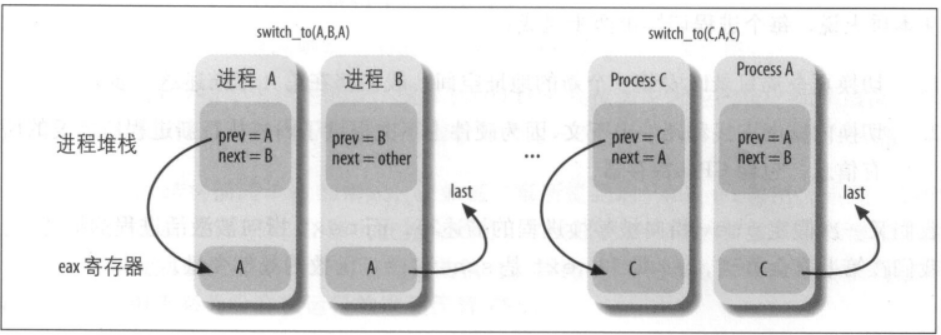
\includegraphics[width=0.8\textwidth]{image/chapter03/通过对进程切换保存对进程C的引用.png}
    \caption{通过对进程切换保存对进程C的引用}
\end{figure}

    由于switch\_to采用扩展内联汇编,因此可读性较差

\begin{itemize}
    \item [1)] 在eax和dx寄存器分别保存prev和next
    \item [2)] 把eflags和ebp寄存器的内容保存在prev内核栈中,因为这些值在更换后不变
    \item [3)] 把esp的内容保存在prev->thread.esp中以使得该字段指向prev内核栈的栈顶
    \item [4)] 把next->thread.esp装入esp,此时内核开始在next的内核栈工作。因此,\emph{改变内核栈意味着改变当前进程。}
    \item [5)] 把标记为1的地址存入prev->thread.eip。当被替换的进程重新恢复时,进程执行被标记为1的指令
    \item [6)] 宏把next->thread.eip的值(绝大多数情况时被标记为1的地址)压入next的内核栈
    \item [7)] 跳转到\_\_switch\_to()函数
    \item [8)] 被进程B替换的进程A再次获得CPU:执行保存eflags和ebp寄存器的指令,这两条指令的第一条指令被标记为1
    \item [9)] 拷贝eax寄存器的内容到switch\_to宏的第三个参数last标识的内存区域中\footnote[1]{\emph{eax寄存器指向刚被替换进程的描述符,当前指向的schedule函数重新使用了prev的局部变量:movl \%eax, prev}}
\end{itemize}

\begin{lstlisting}[language=C++, caption={对于switch\_to的过程描述}]
movl prev, %eax
movl next, %ebx
pushfl
pushl %ebp
movl %esp, 484(%ebp)
movl 484(%edx), %esp
movl $1f, 480(%eax)
pushl 480(%edx)
jmp __switch_to

1: 
    popl %ebp
    popfl
movl %eax, last
\end{lstlisting}

\subsubsection{\_\_switch\_to()函数}

    \_\_switch\_to()函数执行大多数开始于switch\_to宏的进程切换,这个函数作用于prev\_p和next\_p参数,这两个参数标识前一个进程和新进程。为了强迫函数从寄存器中获取参数,内核利用\_\_attribute\_\_和regpram关键字,由gcc编译程序实现

\begin{lstlisting}[language=C++]
struct task_struct fastcall * __switch_to(
    struct task_struct *prev_p, struct task_struct *next_p)
\end{lstlisting}

    函数的执行步骤如下:

\begin{itemize}
    \item 执行由\_\_unlazy\_fpu()宏产生的代码,以有选择地保存prev\_p进程的FPU、MMX和XMM寄存器的内容
    \item 执行smp\_processor\_id()宏获得本地(local)CPU的下标,即执行代码的CPU。
    \item 把next\_p->thread.esp0装入对应于本地CPU的TSS的esp0字段
    \item 把next\_p进程使用的线程局部存储(TLS)段装入本地CPU的全局描述符,三个段选择描述符保存在进程描述符内的tls\_array数组中
    \item 把fs和gs段寄存器的内容分别存放在prev\_p->thread.fs和prev\_p->thread.gs中
    \item 用next\_p->thread.debugreg数组的内容装在dr0,...,dr7中的6个调试寄存器
    \item 如果有必要,更新TSS中的I/O位图。\emph{等next\_p或prev\_p有其自己的定制I/O权限位图时必须这么做}
    \item 终止\_\_switch\_to通过使用返回语句
\end{itemize}

\subsection{保存和加载FPU、MMX及XMM寄存器}

    算术浮点单元(floating-point unit,FPU)被继承到CPU中。MMX用于加速多媒体应用程序的执行,其指令作用于FPU。

    80x86微处理器并不在TSS中自动保存FPU、MMX和XMM寄存器,而是通过硬件支持由cr0寄存器中的一个TS(Task Switching)标志组成,遵循:

\begin{itemize}
    \item 每当执行硬件上下文切换时,设置TS标志
    \item 每当TS标志被设置时,执行ESCAPE、MMX、SSE或SSE2指令,控制单元就产生一个"Device not available"异常
\end{itemize}

    TS标志使得内核只有在真正需要时才保存和恢复FPU、MMX、XMM寄存器。其被描述的数据结构在进程描述符中的thread.i387子字段中:

\begin{lstlisting}[language=C++]
union i387_union {
    struct i387_fsave_struct	fsave;
    struct i387_fxsave_struct	fxsave;
    struct i387_soft_struct soft;
};
\end{lstlisting}

    可以看见,该结构允许选择其中一种结构使用:i387\_soft\_struct由无数学协处理器的CPU模型使用,Linux内核通过软件模拟协处理器来支持这些老式芯片。i387\_fsave\_struct支持协处理器,而最后一种则是支持SSE和SSE2扩展的CPU模型。

    进程描述符包含两个附加的标志:

\begin{itemize}
    \item 包含在thread\_info中的TS\_USEDFPU标志,用于标识当前执行过程中是否使用FPU、MMX和XMM寄存器
    \item 包含在task\_struct中的flags字段中的PF\_USED\_MATH标志。该标志标识thread.i387字段是否有意义
    \subitem 当进程调用execve()时,thread.i387不再有意义
    \subitem 当在用户态执行一个进程执行一个信号处理程序时,不再有意义
\end{itemize}

\subsubsection{保存FPU处理器}

    可以看见,\_\_unlazy\_fpu宏检查prev中的标志位,如果TS\_USEDFPU标志被设置,就说明prev在本次执行中使用了FPU、MMX、SSE或SSE2指令,因此内核需要保存其上下文

\begin{lstlisting}[language=C++]
#define __unlazy_fpu( tsk ) do { \
	if ((tsk)->thread_info->status & TS_USEDFPU) \
		save_init_fpu( tsk ); \
} while (0)
\end{lstlisting}

\begin{itemize}
    \item 把FPU中的内容转储到prev进程描述符中,然后重新初始化FPU。
    \item 重置prev的TS\_USEDFPU标志
    \item 使用stts()宏设置cr0的TS标志
\end{itemize}

\begin{lstlisting}[language=C++]
static inline void __save_init_fpu( struct task_struct *tsk )
{
    if ( cpu_has_fxsr ) {
        asm volatile( "fxsave %0 ; fnclex"
                    : "=m" (tsk->thread.i387.fxsave) );
    } else {
        asm volatile( "fnsave %0 ; fwait"
                    : "=m" (tsk->thread.i387.fsave) );
    }
    tsk->thread_info->status &= ~TS_USEDFPU;
}
\end{lstlisting}

\subsubsection{装载FPU寄存器}

    当next进程刚恢复执行时,浮点寄存器的内容还没有被恢复,因为cr0中的TS标志已被设置,因此next进程第一次试图执行ESCAPE、MMX或SSE/SSE2指令时,控制单元产生"Device not available"异常,内核(异常处理程序)运行math\_state\_restore()函数

\begin{lstlisting}[language=C++]
asmlinkage void math_state_restore(struct pt_regs regs)
{
    struct thread_info *thread = current_thread_info();
    struct task_struct *tsk = thread->task;

    clts();		/* Allow maths ops (or we recurse) */
    if (!tsk_used_math(tsk))
        init_fpu(tsk);
    restore_fpu(tsk);
    thread->status |= TS_USEDFPU; /* So we fnsave on switch_to() */
}
\end{lstlisting}

    该函数清除cr0中的TS标志,且如果thread.i387字段无效,则调用init\_fpu()重新设置该字段,并将PF\_USED\_MATH标志设置为1.

\subsubsection{在内核态使用FPU、MMX和SSE/SSE2单元}

    在内核态使用时,需要注意:

\begin{itemize}
    \item 在使用协处理器之前,如果用户态使用了FPU,内核必须调用kernel\_fpu\_begin(),保存fpu并重置TS标志
    \item 使用完成后,必须使用kernel\_end\_fpu设置TS标志
\end{itemize}

\section{创建进程}

    Unix系统依赖进程创建来满足用户的需求。

    \emph{传统Unix通过统一的方式对待所有进程:子进程复制父进程所有资源。}

    现代Uni引入三种不同的机制解决该问题:

\begin{itemize}
    \item 写时复制技术允许父子进程读相同的物理页。只要二者中有一个试图写一个物理页,内核就把该页的内容拷贝到新页,并分配给正在写的进程
    \item 轻量级进程允许父子进程共享每个进程在内核的数据结构
    \item vfork()创建的进程能共享其父进程的内存地址空间
\end{itemize}

\subsection{clone、fork、vfork系统调用}

    \emph{Linux系统中,轻量级进程由clone()系统调用创建的}:

\begin{itemize}
    \item fn
    \subitem 指定一个由新进程执行的函数
    \item arg
    \subitem 指向传递fn函数的参数
    \item flags
    \subitem clone flags信息
    \item child\_stack
    \subitem 把用户态堆栈指针赋值给子进程的esp寄存器,调用进程应该总是为子进程分配新的堆栈
    \item tls
    \subitem 表示线程局部存储段(TLS)的地址,只有CLONE\_SETTLS标志有效才有意义
    \item ptid
    \subitem 表示父进程的用户态变量地址,该父进程具有与新轻量级进程一样的PID,只有在CLONE\_PARENT\_SETTID有效才有意义
    \item ctid
    \subitem 表示轻量级进程用户态变量地址,只有CLONE\_CHILD\_SETTID标志有效才有意义
\end{itemize}

\begin{lstlisting}[language=C++, caption={clone flags}]
/* set if VM shared between processes */
#define CLONE_VM	0x00000100	
/* set if fs info shared between processes */
#define CLONE_FS	0x00000200	
/* set if open files shared between processes */
#define CLONE_FILES	0x00000400	
/* set if signal handlers and blocked signals shared */
#define CLONE_SIGHAND	0x00000800	
/* set if we want to let tracing continue on the child too */
#define CLONE_PTRACE	0x00002000	
/* set if the parent wants the child to wake it up on mm_release */
#define CLONE_VFORK	0x00004000	
/* set if we want to have the same parent as the cloner */
#define CLONE_PARENT	0x00008000	
/* Same thread group? */
#define CLONE_THREAD	0x00010000	
/* New namespace group? */
#define CLONE_NEWNS	0x00020000	
/* share system V SEM_UNDO semantics */
#define CLONE_SYSVSEM	0x00040000	
/* create a new TLS for the child */
#define CLONE_SETTLS	0x00080000	
/* set the TID in the parent */
#define CLONE_PARENT_SETTID	0x00100000	
/* clear the TID in the child */
#define CLONE_CHILD_CLEARTID	0x00200000	
/* Unused, ignored */
#define CLONE_DETACHED		0x00400000	
/* set if the tracing process can't force CLONE_PTRACE on this clone */
#define CLONE_UNTRACED		0x00800000	
/* set the TID in the child */
#define CLONE_CHILD_SETTID	0x01000000	
/* Start in stopped state */
#define CLONE_STOPPED		0x02000000	
\end{lstlisting}

    事实上,clone是C语言库中的一个封装函数,负责建立新轻量级进程的堆栈并且调用对编程者隐藏的clone系统调用。

    实现clone的sys\_clone服务例程没有fn和arg参数。封装函数把fn指针放在子进程堆栈中的某个位置,该位置就是该封装函数本身返回地址存放的位置。arg指针正好存放在子进程堆栈中fn的下方

    传统的fork系统调用是由clone实现的,其中clone的flags参数指定为SIGCHLD信号及所有清零的clone标志,child\_stack由父进程当前的堆栈指针。因此,父子进程暂时共享一个用户态堆栈(但是由于写时拷贝机制,通常只要其中一个进程更改栈,就会立即得到各自的用户态堆栈拷贝)

\begin{lstlisting}[language=C++]
long sys_clone(
    unsigned long clone_flags, unsigned long newsp,
    int __user *parent_tid, int unused, int __user *child_tid)
\end{lstlisting}